After establishing a theoretical foundation both about multigrid methods and evolutionary grammar-based optimization techniques, the first primary goal of this thesis is to develop a formal language for expressing arbitrarily structured multigrid solvers in a generalized way.
For this purpose, first observe that the multigrid solvers described Section~\ref{sec:multigrid-cycles} can be all classified by their \emph{cycle type}.
Each such cycle possesses a distinct computational pattern which stems from the number of recursive descents performed on each level of the method.
For instance a V-cycle is characterized by exactly one recursive descent per level.
All these classically considered multigrid cycles employ a fixed uniform number of recursive descents and smoothing steps per discretization level, which is determined by the parameters $\gamma$, $\nu_1$ and $\nu_2$ in Algorithm~\ref{alg:multigrid-cycle}.
While the representation of a multigrid method as a recursive cycle yields a formally simple and easily parameterizable algorithmic formulation it also enforces unnecessary restrictions on its structure.
Consider for instance the multigrid method depicted in Figure~\ref{fig:non-traditional-multigrid-cycle}.
\begin{figure}
	\begin{subfigure}{0.1\textwidth}
		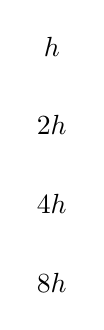
\begin{tikzpicture}
			\node   (h) at (-0.75, 4){$h$};
			\node   (2h) at (-0.75, 3){$2h$};
			\node   (4h) at (-0.75, 2){$4h$};
			\node   (8h) at (-0.75, 1){$8h$};
		\end{tikzpicture}
	\end{subfigure}
	\begin{subfigure}{0.9\textwidth}
		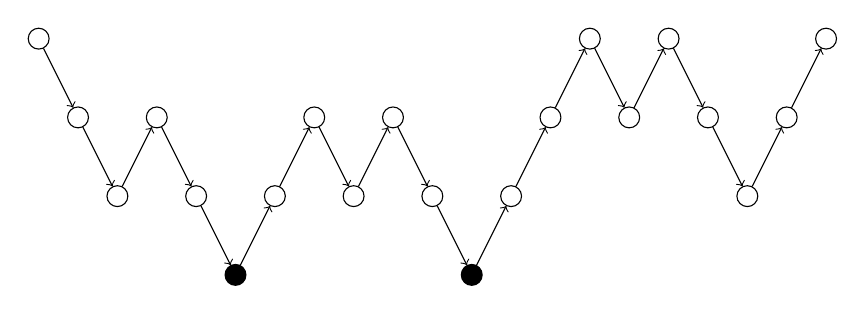
\begin{tikzpicture}
			\node	(a) at (0,4) [draw, circle,scale=0.8] {};
			\node	(b) at (0.5,3) [draw, circle,scale=0.8] {};
			\node	(c) at (1,2) [draw, circle,scale=0.8] {};
			\node	(d) at (1.5,3) [draw, circle, scale=0.8] {};
			\node	(e) at (2,2) [draw, circle, scale=0.8] {};
			\node	(f) at (2.5,1) [draw, circle,scale=0.8,fill=black] {};
			\node	(g) at (3,2) [draw, circle,scale=0.8] {};
			\node	(h) at (3.5,3) [draw, circle,scale=0.8] {};
			\node	(i) at (4,2) [draw, circle,scale=0.8] {};
			\node	(j) at (4.5,3) [draw, circle,scale=0.8] {};
			\node	(k) at (5,2) [draw, circle,scale=0.8] {};
			\node	(l) at (5.5,1) [draw, circle,scale=0.8,fill=black] {};
			\node	(m) at (6,2) [draw, circle,scale=0.8] {};
			\node	(n) at (6.5,3) [draw, circle,scale=0.8] {};
			\node	(o) at (7,4) [draw, circle,scale=0.8] {};
			\node	(p) at (7.5,3) [draw, circle,scale=0.8] {};
			\node	(q) at (8,4) [draw, circle,scale=0.8] {};
			\node	(r) at (8.5,3) [draw, circle,scale=0.8] {};
			\node	(s) at (9,2) [draw, circle,scale=0.8] {};
			\node	(t) at (9.5,3) [draw, circle,scale=0.8] {};
			\node	(u) at (10,4) [draw, circle,scale=0.8] {};
			\draw 
			(a) edge[->] (b) 
			(b) edge[->] (c)
			(c) edge[->] (d)
			(d) edge[->] (e)   
			(e) edge[->] (f)
			(f) edge[->] (g)
			(g) edge[->] (h)
			(h) edge[->] (i)
			(i) edge[->] (j)
			(j) edge[->] (k)
			(k) edge[->] (l)
			(l) edge[->] (m)
			(m) edge[->] (n)
			(n) edge[->] (o)
			(o) edge[->] (p)
			(p) edge[->] (q)
			(q) edge[->] (r)
			(r) edge[->] (s)
			(s) edge[->] (t)
			(t) edge[->] (u)
			;
		\end{tikzpicture}
	\end{subfigure}
	\caption{Example for a non-traditional multigrid method.}
	\label{fig:non-traditional-multigrid-cycle}
\end{figure}
While this method reaches the coarsest level twice and, hence, at first sight looks similar to a W-cycle, it employs a unique pattern of computations that is completely different from those of any of the traditional multigrid cycles.
As a consequence, this method can not be represented within the classical framework of multigrid cycles, as formulated in Algorithm~\ref{alg:multigrid-cycle}.
To overcome these limitations and construct multgrid methods with an arbitrary sequence of computations on each discretization level, as illustrated by the example in Figure~\ref{fig:non-traditional-multigrid-cycle}, a new formal language for their representation is needed.
The first step towards the development of this language is to find a way to represent the current state within each step of a multigrid method and then define transition rules between those states.
\section{Multigrid States and Transitions}



